\documentclass[tikz]{standalone}


\usetikzlibrary{math,decorations.pathreplacing,calc,decorations.markings}
\tikzset{->-/.style={decoration={
			markings,
			mark=at position {0.5*\pgfdecoratedpathlength+.5*3pt} with {\arrow{>}}},postaction={decorate}}}
\tikzset{-<-/.style={decoration={
			markings,
			mark=at position {0.5*\pgfdecoratedpathlength+.5*3pt} with {\arrow{<}}},postaction={decorate}}}

\begin{document}

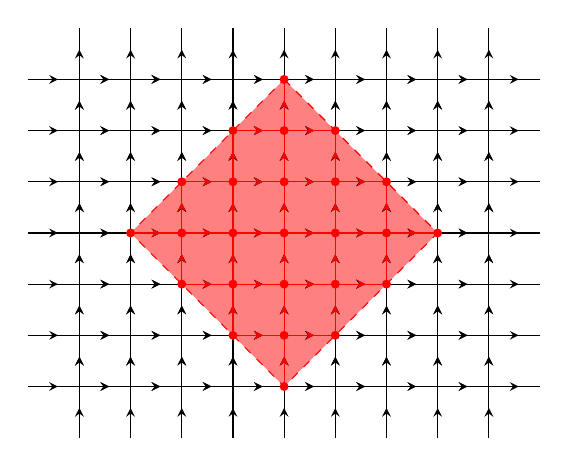
\begin{tikzpicture}[>=stealth, scale=0.65]
	\draw[red,dashed,fill=red!50] (0,3) -- (3,0) -- (0,-3) -- (-3,0) -- cycle;
	
	\foreach \i in {-4,...,4} {
		\foreach \j in {-3,...,3} {
			\draw[->-] (\i,\j) -- ({\i+1},{\j});
			\draw[->-] (\i,\j) -- ({\i},{\j+1});
			\draw[->-] ({\i-1},\j) -- (\i,\j);
			\draw[->-] (\i,{\j-1}) -- (\i,\j);
		};
	};
	\fill[red] ( 0, 0) circle (2.5pt);
	
	\fill[red] ( 1, 0) circle (2.5pt);
	\fill[red] (-1, 0) circle (2.5pt);
	\fill[red] ( 0, 1) circle (2.5pt);
	\fill[red] ( 0,-1) circle (2.5pt);
	
	\draw[red,->-] ( 0, 0) -- ( 1, 0);
	\draw[red,->-] (-1, 0) -- ( 0, 0);
	\draw[red,->-] ( 0, 0) -- ( 0, 1);
	\draw[red,->-] ( 0,-1) -- ( 0, 0);
	
	\fill[red] ( 2, 0) circle (2.5pt);
	\fill[red] (-2, 0) circle (2.5pt);
	\fill[red] ( 0, 2) circle (2.5pt);
	\fill[red] ( 0,-2) circle (2.5pt);
	
	\fill[red] ( 1, 1) circle (2.5pt);
	\fill[red] ( 1,-1) circle (2.5pt);
	\fill[red] (-1, 1) circle (2.5pt);
	\fill[red] (-1,-1) circle (2.5pt);
	
	\draw[red,->-] ( 1, 0) -- ( 2, 0);
	\draw[red,->-] (-2, 0) -- (-1, 0);
	\draw[red,->-] ( 0, 1) -- ( 0, 2);
	\draw[red,->-] ( 0,-2) -- ( 0,-1);
	
	\draw[red,->-] ( 0, 1) -- ( 1, 1);
	\draw[red,->-] (-1, 1) -- ( 0, 1);
	\draw[red,->-] ( 0,-1) -- ( 1,-1);
	\draw[red,->-] (-1,-1) -- ( 0,-1);
	
	\draw[red,->-] ( 1, 0) -- ( 1, 1);
	\draw[red,->-] ( 1,-1) -- ( 1, 0);
	\draw[red,->-] (-1, 0) -- (-1, 1);
	\draw[red,->-] (-1,-1) -- (-1, 0);
	
	\fill[red] ( 3, 0) circle (2.5pt);
	\fill[red] (-3, 0) circle (2.5pt);
	\fill[red] ( 0, 3) circle (2.5pt);
	\fill[red] ( 0,-3) circle (2.5pt);
	
	\fill[red] ( 1, 2) circle (2.5pt);
	\fill[red] ( 2, 1) circle (2.5pt);
	\fill[red] ( 1, -2) circle (2.5pt);
	\fill[red] ( 2, -1) circle (2.5pt);
	\fill[red] ( -1, 2) circle (2.5pt);
	\fill[red] ( -2, 1) circle (2.5pt);
	\fill[red] ( -1, -2) circle (2.5pt);
	\fill[red] ( -2, -1) circle (2.5pt);
	
	\draw[red,-<-] ( 1, 2) -- +( 0,-1);
	\draw[red,-<-] ( 1, 2) -- +(-1, 0);
	\draw[red,-<-] ( 2, 1) -- +( 0,-1);
	\draw[red,-<-] ( 2, 1) -- +(-1, 0);
	
	\draw[red,-<-] (-1, 2) -- +( 0,-1);
	\draw[red,->-] (-1, 2) -- +( 1, 0);
	\draw[red,-<-] (-2, 1) -- +( 0,-1);
	\draw[red,->-] (-2, 1) -- +( 1, 0);
	
	\draw[red,->-] ( 1,-2) -- +( 0, 1);
	\draw[red,-<-] ( 1,-2) -- +(-1, 0);
	\draw[red,->-] ( 2,-1) -- +( 0, 1);
	\draw[red,-<-] ( 2,-1) -- +(-1, 0);
	
	\draw[red,->-] (-1,-2) -- +( 0, 1);
	\draw[red,->-] (-1,-2) -- +( 1, 0);
	\draw[red,->-] (-2,-1) -- +( 0, 1);
	\draw[red,->-] (-2,-1) -- +( 1, 0);
	
	\draw[red,-<-] ( 3, 0) -- +(-1, 0);
	\draw[red,->-] (-3, 0) -- +( 1, 0);
	\draw[red,-<-] ( 0, 3) -- +( 0,-1);
	\draw[red,->-] ( 0,-3) -- +( 0, 1);
	
\end{tikzpicture}
\end{document}